{\color{gray}\hrule}
\begin{center}
\section{Technical Approach}
%\textbf{bla bla }
\end{center}
{\color{gray}\hrule}


\begin{multicols}{2}
In order to get across the inner workings of each module we will separate this section into subsections related to each one.

\subsection{Pre-processing}
As the objective of the system is to be adaptable to dirty and noisy input images, in the pre-processing phase great care should be taken to clean such inputs. As such the pre-processing module applies different methods of input refinement in sequence.

A first denoising pass is performed utilizing the bilateral filter, after which the image goes through a light adjustment procedure which entails contrast stretching.

After these operations we perform the background removal. This is because we thought that a potential point of improvement within the virtual try-on pipeline could be the removal of the background before going deeper into the pipeline, as the background information may hinder the performance of the subsequent modules. To perform such a task we are looking and comparing multiple already existing solutions such as:
\begin{itemize}
\item U-Net\cite{u-net} fine-tuning a pre-trained U-Net model using the \textit{Full Body TikTok Dancing Dataset}\cite{tik_tok_dataset};

\item Detectron2\cite{detectron2}: fine-tuning on \textit{Full Body TikTok Dancing Dataset} the Detectron2 segmentation module released by Facebook;

\item Detectron2 + GrabCut: We also tried to enhance the results of Detectron2 predictions by adding a post-processing layer where the output is used as a GrabCut initializing region; then we applied a median filter to smooth the edges. This was done in an attempt to better fit the segmantion done by Detectron2 to the shape of the body.
\end{itemize}

We will compare the results and choose the best one according to state-of-the-art evaluation metrics (IoU, DICE etc...).



\subsection{Person representation}
This module deals with the semantic segmentation of the subject and their keypoints extraction, which will be used to as features for the warping module.

Regarding the segmentation problem we have, as of now, identified the Detectron2 segmentation module as the main candidate to solve it.

Instead, for the keypoint extraction problem we are comparing the DensePose module (from Detectron2) and the OpenPose module.

\end{multicols}

\begin{figure*}[h]
\centering
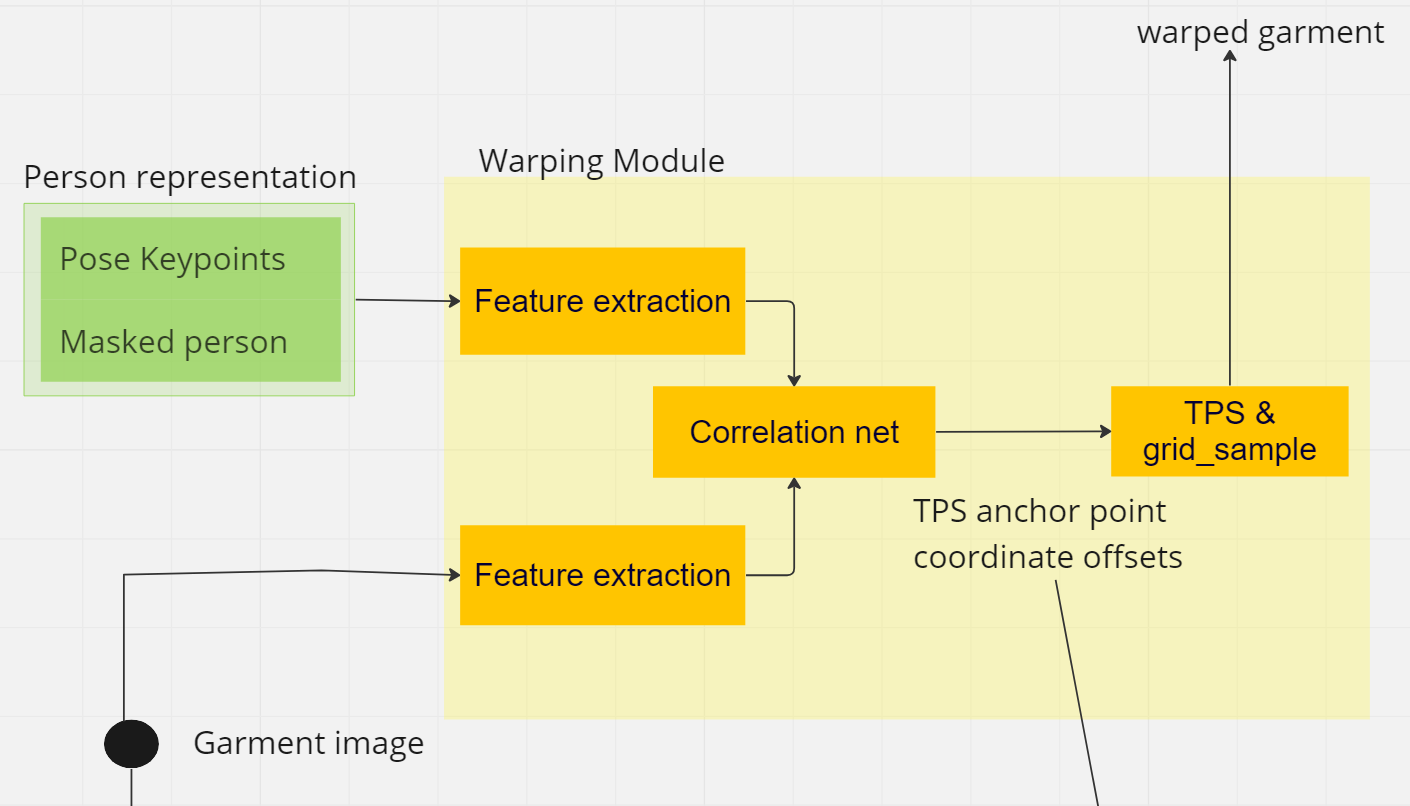
\includegraphics[scale=0.4]{warping_module_schema}
\caption{Warping module schema}
\label{fig:warp_schema}
\end{figure*}

\begin{figure*}[h]
\centering
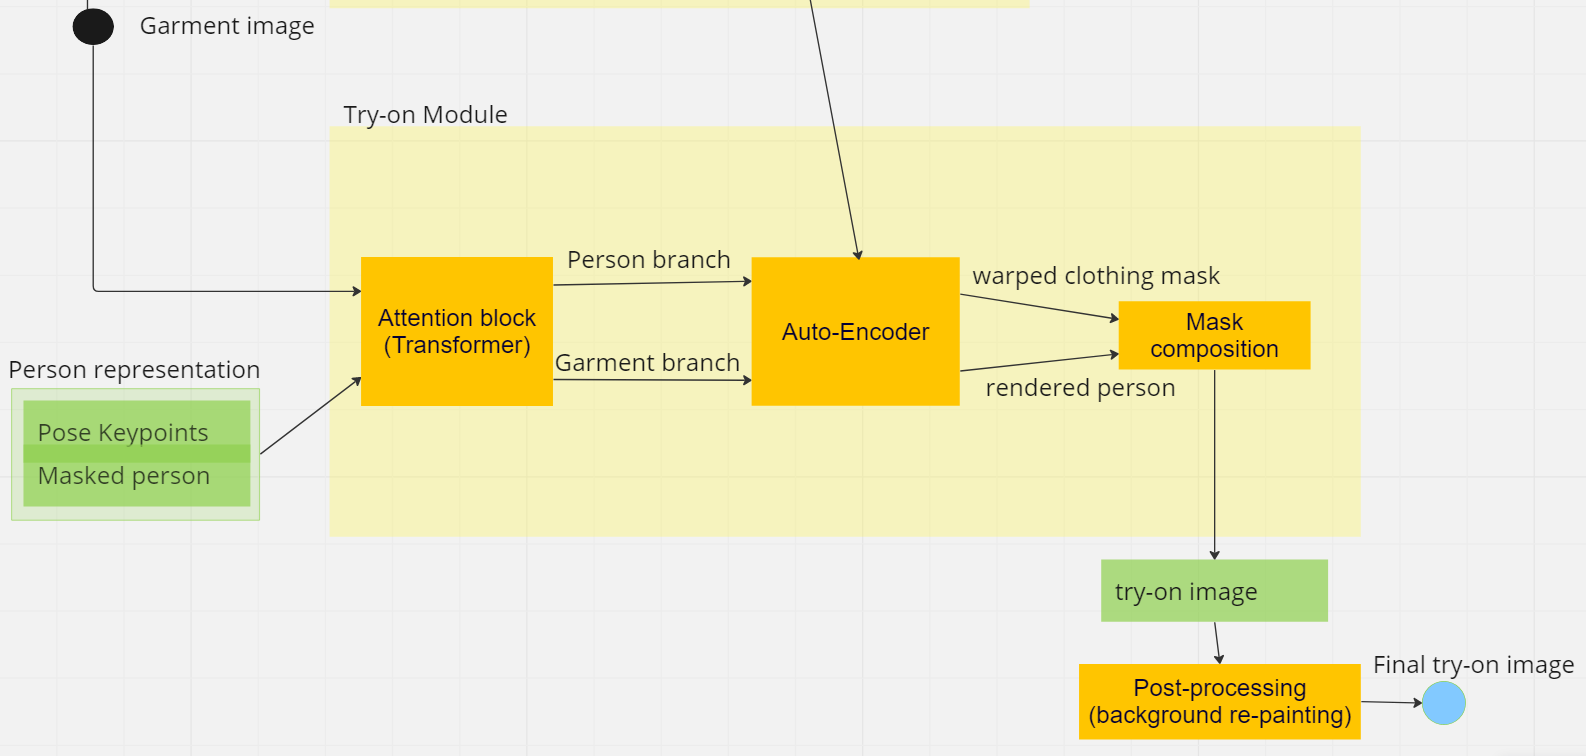
\includegraphics[scale=0.5]{generative_module}
\caption{Generative module schema}
\label{fig:gen_schema}
\end{figure*}

\begin{multicols}{2}

\subsection{Warping module}
As depicted in the figure \ref{fig:warp_schema}, the warping module takes as inputs the person representation feature vector and the garment image and, based on the keypoints and the segmantation mask, it warps the garment fitting it to the body shape of the subject.

The output is the set of the TPS parameters, which are used to geometrically transform the clothing item.



\subsection{Generative module}
As depicted in the figure \ref{fig:gen_schema}, the generative module is the one which will be producing the final image by merging the warped garment with the human picture.

The module will consist of a transformer-based feature extraction unit which will feed into an autoencoder unit which will generate the output image.




\subsection{Garment Retrieval}
The garment retrieval module will be handling the image retrieval part of our system. The garment retrieval will be comparing the query images by evaluating the similairty between the extracted descriptors and the reference descriptors (stored in the repository). 

The first task will be choosing and comparing different feature extraction algorithm which will define the image descriptors.

After the selection we will have to build our garment repository, which will be composed of the compressed descriptors extracted from each reference image.

Finally, the system will be able to compute the input image descriptor and compare it to the descriptors stored in the repository and retrieve the best matches, based on a chosen similarity function.




\end{multicols}